%%%  Vzor pro použití makra pro diplomovou práci
%%%  (c) Miloš Kudělka, David Skoupil, březen 1998
%%%  Vzorový soubor revidován a doplněn v září 2001
%%%  (c) 2001 Vilém Vychodil, <vilem.vychodil@upol.cz>
%%%  Vzorový soubor upraven v květnu 2009
%%%  (c) 2009 Jan Outrata, <jan.outrata@upol.cz>
%%%
%%%  Po přeložení programem CSLaTeX (třikrát) je potřeba použít
%%%  program DVIPS a takto získaný PostScriptový soubor vytisknout
%%%  na PostScriptové tiskárně nebo pomocí programu GhostScript.
%%%
%%%  Rovněž je možné použít program DVIPDFM a vytvořit z dokumentu
%%%  soubor ve formátu PDF včetně hypertextových odkazů.


%%% Deklarace hlavičky dokumentu, použijte písmo velikosti 12 bodů.
\documentclass[12pt]{article}

%%% Připojení dodatečného stylu pro diplomové práce. V případě
%%% (magisterské) diplomové práce použijte nepovinný argument
%%% `master', který zajistí vysázení správného označení práce
%%% ``DIPLOMOVÁ PRÁCE'' na titulní straně (výchozí je ``BAKALÁŘSKÁ
%%% PRÁCE'').
%%%
%%% Nepovinné argumenty `tables' a `figures' použijte pouze v případě,
%%% že váš dokument obsahuje tabulky a obrázky a chcete vytvořit
%%% jejich seznamy za obsahem.
%%%
%%% Argument `joinlists' způsobí zřetězení obsahu a seznamů tabulek a obrázků.
%%% Není-li použít, všechny seznamy jsou uvedeny na samostatných stránkách.
%%%
%%% Pokud chcete vytvářet pouze dokument ve formátu PostScript, můžete uvést
%%% dodatečný argument `nopdf'. Tím se potlačí chybová hlášení při použití
%%% programu `dvips'.
\usepackage[tables,figures]{updiplom}

%%% Dodatečné standardní styly.
\usepackage[utf8]{inputenc}
\usepackage{subfigure}
\usepackage{acronym}

% Definovane zkratky
\acrodef{ACO}{Ant Colony Optimization}
\acrodef{AS}{Ant System}
\acrodef{S-ACO}{Simple Ant Colony Optimization}
\acrodef{TDD}{Test Driven Development}




%%% Parametry pro vytvoření úvodních stránek. Makrem \subtitle je možné
%%% vytvořit druhý řádek v názvu diplomové práce.
\title{Samoučící algoritmus pro deskové hry}
%\subtitle{Druhý řádek názvu diplomové práce}
\author{Vojtěch Šalbaba}
\year{2010}
\date{9. květen 2010}

%%% Pomocí \docinfo je možné vytvořit název pro PDF dokument, zpravidla je
%%% dobré použít předcházející název, ale bez diakritiky. Možné je však zvolit
%%% úpolně jiný výstižný název. Při tvorbě PostScriptu bude příkaz ignorován.
\docinfo{Vojtech Salbaba}{Samoucici algoritmus pro deskove hry}

%%% Vytvoření anotace. Pouze jeden odstavec!
\annotation{%
Záměrem práce je prozkoumat fungování, možnosti, vlastnosti, výhody a omezení algoritmů z rodiny Ant Colony Optimization, posléze jeden z nich aplikovat na problém nalezení nejlepšího tahu v jednoduché deskové hře a porovnat jeho výkon s algoritmem MiniMax.
}

%%% Nepovinný text poděkování. Pouze jeden odstavec!
\thanks{%
Poděkování vedoucímu práce, rodině apod. (nepovinné)
}

\begin{document}

%%% Vytvoření úvodních stránek, obsahu a seznamu tabulek a obrázků.
\maketitle
\newpage

%%% Text diplomové práce.
\medskip
\section{Úvod do Ant Colony Optimization}
\subsection{Chování mravenců v přírodě}
\begin{quotation}
Mravenci v přírodě vykazují chování, které již dlouhou dobu přitahuje lidskou pozornost. Pravděpodob\v{n}ě jedním z nejvíce pozoruhodných chování je vytváření tzv. cestiček. Když jsme byli mladí, mnoho z nás šláplo na takovouto \uv{dálnici} nebo na ni položili překážku jen abychom viděli jak mravenci zareagují na takovéto vyrušení. Zárove\v{n} jsme uvažovali kam tyto cesty vedou a nebo jak vlastně vznikají. Jak vyrůstáme, přestávají nás takovéto otázky zajímat - existuje ale nezanedbatelný počet výzkumníků, především biologů, kteří toto chování podrobně studují. \cite{dorigo2004}
\end{quotation}
Komunikace mravenců je obecně velmi zajímavá. Ke komunikaci nepoužívají audiovizuální komunikaci jako lidé, ale pachové stopy, zanechávané v prostředí. Chování jednotlivých mravenců můžeme jednoduše popsat a pochopit - mravenec při chůzi klade feromony a je jimi přitahován. Chování celé kolonie, které je určeno jednoduchým chováním jednotlivců, je naopak velmi komplexní. Můžeme ho přirovnat k chování Langtonova mravence. 

Langtonův mravenec je na první pohled velmi jednoduchý konstrukt. Představme si, že na nekonečné 2 rozměrné čtvercové síti se pohybuje mravenec. Předpokládejme, že čtverce mohou být buď bílé nebo černé. Pokud se mravenec nachází na černém poli, přebarví ho na bílé a přesune se pole vpravo od něj. Pokud se nachází na bílém, přebarví ho na černé a přesune se pole vlevo od něj. Jeho chování můžeme jednoduše popsat a pochopit, stejně jako chování jednotlivého mravence. Ale jak se bude takový mravenec chovat? Chování, které u něj pozorujeme, se dá rozdělit do 3 fází.
\begin{description}
\item[Jednoduchost] 
Prvních 200--300 kroků mravenec začínající na kompletně bílé ploše vytváří jednoduché a často symetrické tvary. Jeho chování se nám zdá zřejmé, jednoduchá pravidla generují jednoduché obrazce.

\item[Chaos]
Pak od nějakého bodu přestanou mít obrazce které vytváří zřejmou strukturu, a zdají se náhodné. Tato fáze trvá přibližně $10000$ kroků. Pokud tedy nemáme dostatečně výkonou techniku, můžeme pozorování po nějaké době vzdát s pocitem, že se už nic zajímavého nestane. Sice víme, že mravenec se řídí stejnými pravidly jako předtím, ale \uv{z dálky to tak nevypadá}.

\item[Pořádek] Nakonec se mravenec dostane do jakési smyčky, a začne stavět cestu. Prochází cyklem 104 kroků, po kterých se posune o 2 kroky šikmo a čtverce okolo jsou stejných barev jako na počátku cyklu. 
\end{description}

\begin{figure}[hbtp]
  \caption{Langtonův mravenec}
  \label{fig:langtonant}
  \begin{center}
  	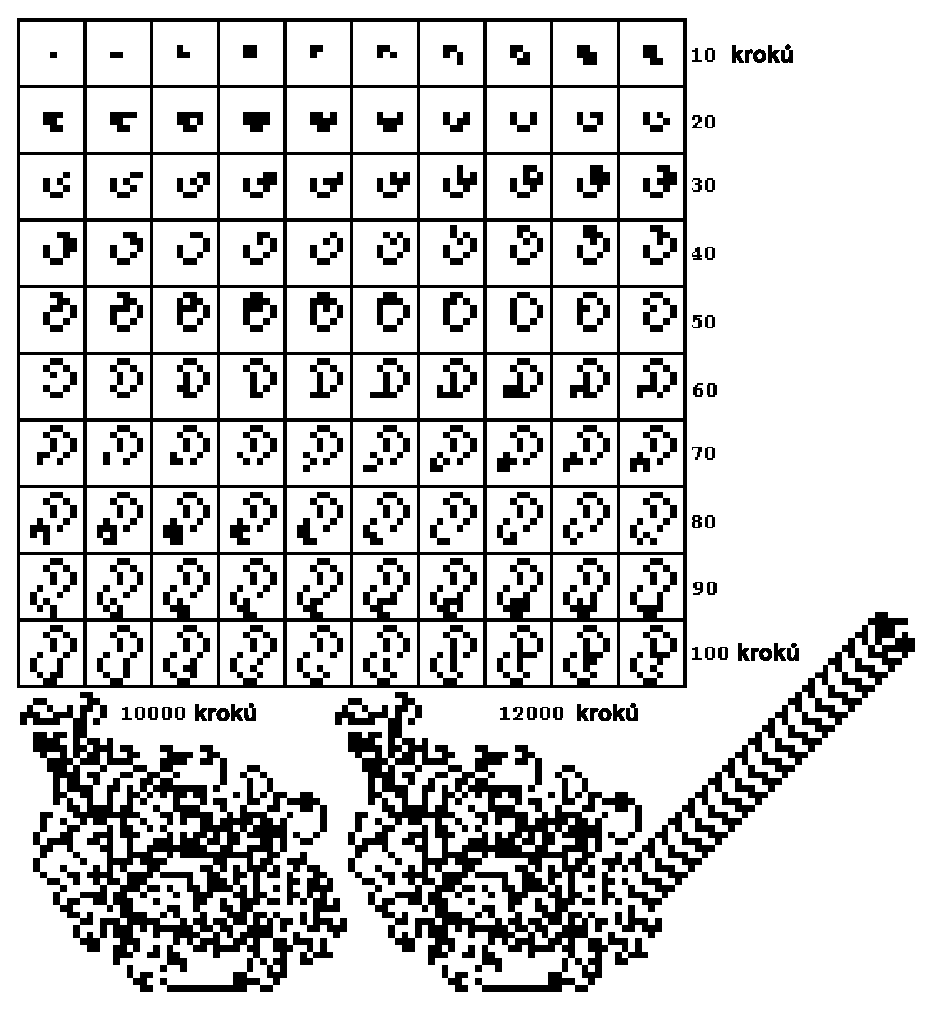
\includegraphics[scale=0.5]{AMEIHUND_Langtons_Ameise_svensk}
  \end{center}
\end{figure}

Toto je pro nás nečekané, a těžko předvídatelné z nám známých 2 jednoduchých pravidel pro chování Langtonova mravence. Všechny 3 fáze vychází ze stejných pravidel, ale jediný způsob jak z pravidel \uv{bílá doleva, černá doprava} odvodit výsledek \uv{staví cestu} je nechat mravence běžet. Stejně tak chování které vznikne z interakce mnoha skutečných mravenců, kteří jsou samostatně jednoduší, je zřejmé teprve z delšího pozorování celé kolonie.\cite{prattchet2002}

\subsection{Experiment dvou větví}

\begin{figure}[htbp]\caption{Varianty experimentu dvou větví} \label{fig:doublebridgevariants}
	\begin{center}
		\subfigure[Stejně dlouhé větve]{\label{fig:simpledoublebridge}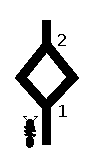
\includegraphics[scale=2]{simple_double_bridge}}
		\subfigure[Poměr větví 1:2]{\label{fig:doublebridge}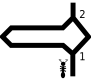
\includegraphics[scale=2]{double_bridge}}
		\subfigure[Kratší větev přidána později]{\label{fig:attachingdoublebridge}\includegraphics[scale=2]{attaching_double_bridge}}
	\end{center}
\end{figure}

Chování skutečných mravenčích kolonií jako celku lze dobře demonstrovat na \emph{experimentu dvou větví}. Experiment je položen takto: Mravenci jsou od jídla odděleni mostem, který se rozdvojuje a zase spojuje, viz. obrázek \ref{fig:simpledoublebridge}. Obě větve mostu jsou stejně dlouhé. Jak mravenci cestují po mostu, každý z nich zanechává za sebou feromony, které ovlivňují pravděpodobnost, že ostatní mravenci vyberou právě jeho cestu. Tak vzniká pozitivní zpětná vazba, která po počátečních výkyvech velmi rychle vede k tomu, že jedna cesta je kompletně opuštěna. Tato konvergence k jedné cestě trvá u kolonií zhruba 10--25 minut. \cite{deneubourg1989}

Pozmě\v{n}me experiment tak, že jedna větev mostu je 2x delší než druhá, a cesta po delší větvi tedy trvá mravenci 2x tak dlouho, jako na obrázku \ref{fig:doublebridge}. Mravenci, kteří se vydají kratší cestou, se vrátí do mraveniště dříve, a zůstanou po nich tedy feromony na cestě \emph{tam i zpátky}. Než se vrátí mravenci, kteří zvolili delší cestu, je na cestách použitých dříve se navrátivšími mravenci $2\times$ více feromonů a díky pozitivní zpětné vazbě bude kratší cesta brzo silně preferována. Lze odvodit, že druhy mravenců, které nezanechávají feromony po cestě tam i zpět, nemohou uspět ve výběru kratší cesty jinak než čirou náhodou.

Udělejme další změnu experimentu. Mravencům představíme jen jednu cestu, a po nějakém čase po objevení jídla na jejím druhém konci k ní přidáme kratší alternativu (obrázekk \ref{fig:attachingdoublebridge}). Mravenci se díky pozitivní zpětné vazbě nemohou dostat z jejich již nalezené dlouhé cesty a nedojde k přechodu na kratší cestu. \cite{goss1989}

Toto chování, kdy mravenci nenajdou nově se objevivší lepší alternativu, je způsobeno tím, že zatímco mravenci se pro jednu cestu rozhodnou za zhruba 10--25 minut, feromony vyprchají po více jak půlhodině. Vyprchávání feromonů tedy je pro simulaci zanedbatelné. \cite{deneubourg1989}

\subsection{Simulace experimentu dvou větví}
Přírodní prostředí si představme jako graf $G = (U, H)$, kde vrcholy $U, n = |U|$ představují místa kde mravenci musí volit a hrany $H$ cesty mezi nimi. Vzdálenost mezi dvěma místy převedeme na ohodnocení odpovídajích hran nebo počet uzlů (obě reprezentace vzdálenosti jsou ekvivalentní). Mraveniště budeme reprezentovat jedním z vrcholů grafu $G$ a budeme ho nazývat \emph{zdroj}. Potravu budeme reprezentovat dalším vrcholem grafu $G$ a budeme ho nazývat \emph{cíl}. Zatímco v reálném světě je čas spojitá veličina, my ji budeme reprezentovat jako diskrétní veličinu $t = 1, 2, ...$ a v každém kroku času mravenci pohnou o jednu vzdálenostní jednotku. Mravenci si další krok volí na základě pravděpodobnosti: $p_{ih}(t)$ je pravděpodobnost, že mravenec v čase $t$ ve vrcholu $i$ si vybere hranu $h$. $\varphi_{ia}(t)$ je počet feromonů na hraně $a$ z vrcholu $i$.

\begin{equation}\label{abstraktprob}
p_{h}(t)=\frac{\left[ \varphi_{h}(t) \right]^\alpha }{ \sum_{h} \left[ \varphi_{ih} \right]^\alpha}
 \end{equation}
 
kde $\sum_{h}\varphi_{ih}$ znamená \uv{součet feromonů na všech hranách vycházejících z uzlu $i$} a $\alpha$ je volený parametr. Pokud hrana $h$ vede z vrcholu $i$ do vrcholu $j$, pak $\varphi_{ih}$ je rovno

\begin{equation}\label{abstraktphi}
\varphi_{ih}(t) = p_{ih}(t-1)*m_i(t-1) + p_{jh}(t-1)*m_j(t-1)
 \end{equation}
 
kde $m_i(t)$ je počet mravenců ve vrcholu $i$ v čase $t$. 

Tento způsob abstrakce je velmi přímočarý, mezi jeho výhody patří především převedení času ze spojitého na diskrétní, a také že nepracuje přímo s jednotlivými mravenci ale s průměrným chování celé kolonie. Podrobnější diskuzi s příklady lze nalézt v \cite{maniezzo2004}.

\subsection{Simple Ant Colony Optimization}
Předchozí abstrakce nám posloužila dobře pro pochopení problému se dvěma větvemi, ale zřejmě není vhodná pro aplikaci na složitější problémy. Nepracuje totiž dobře s grafy obsahujícími kružnice, kde mravenci jednoduše uváznou. Proto zavedeme nové procesy - eliminaci kružnic a vyprchávání feromonů. Výsledkem bude algoritmus \ac{S-ACO}.

Pro jednoduchost budeme vzdálenost převádět na počet uzlů oddělující dva body, nikoli na ohodnocení cest. Označme proces cesty mravence od zdroje k cíli jako \emph{dopřednou aktualizaci}, a jeho návrat od cíle k zdroji jako \emph{zpětnou aktualizaci}. Rozšiřme zárove\v{n} schopnosti každého mravence o pamě\v{t} vrcholů, které navštívil za jeho cestu od zdroje k cíli a hran, které k tomu použil. Dále zaveďme funkci $\tau_{ij}$, která pro $\forall i, j \in U$ přiřadí počet feromonů a funkci $S_{i}^{k}$, která mravenci $k$ přiřadí množinu sousedních uzlů uzlu $i$ takovou, že v ní není zahrnut uzel, ze kterého mravenec $k$ do uzlu $i$ přišel. Pokud by $O^k_i$ měla být prázdná, mravenci návrat povolíme. Pravděpodobnost, že mravenec $k$ vybere konkrétní cestu $ij$ pak spočteme jako 
\begin{equation}\label{sacopravdepodobnost}
p_{ij}^k = \frac{\tau_{ij}^\alpha}{\sum_{l \in S_{i}^k} \tau_{il}^\alpha}
\end{equation}
pokud $j \in O_{i}^{k}$, jinak $0$. Konstantu $\alpha$ volíme $\geq 1$, a tato konstanta ovlivní rychlost konvergence kolonie k jedné z cest.

V předchozím modelu mravenci ukládali feromony v průběhu dopředné i zpětné aktualizace. Upravíme chování našich mravenců tak, že při dopředné aktualizaci sice vybírají hrany, které použijí s ohledem na feromony, které na nich leží, ale \emph{sami feromony neukládají}. Místo toho si pouze pamatují použitou cestu. Po dosažení cíle potom přejdou do fáze zpětné aktualizace, ve které se budou chovat deterministicky - půjdou zpět po zapamatované cestě, ze které ale nejdříve odstraníme kružnice. Z kvality cesty po odstranění kružnic pak mravenec určí počet feromonů, které na ni uloží. Pokládání feromonů lze zapsat jako
\begin{equation}\label{sacoaktualizce}
\tau_{ij} \leftarrow \tau_{ij} + \Delta\tau^k
\end{equation} 
Kvalita výsledků \ac{S-ACO} závisí na volbě způsobu výpočtu $\Delta\tau^{k}$. Můžeme zvolit například konstantní funkci, nebo v ní promítnout kvalitu cesty, například $\Delta\tau^k = \frac{1}{L^{k}}$, kde $L^{k}$ je délka cesty mravence $k$. \cite{maniezzo2004} ukazuje, že kolonie se $\Delta\tau^k$ zohled\v{n}ující kvalitu cesty potřebují pro nalezení řešení nižší počet mravenců.

Zatímco dříve jsme při simulaci opravdových mravenčích kolonií zanedbávali vliv vyprchávání feromonů, nyní tuto vlastnost použijeme pro získání lepších výsledků. Vyprcháváním feromonů budeme přikládat menší váhu řešením nalezeným na začátku běhu, která vznikla když kolonie ještě neměla dostatek informací pro vytvoření optimální cesty. Vyprchávání feromonů provedeme tak, že po tom, co se všichni mravenci pohnou do dalšího vrcholu, ze všech cest vyprchá poměrná část feromonů
\begin{equation}\label{sacovyprchavani}
\tau_{ij} \leftarrow (1 - \rho)\tau_{ij}, \rho \in \left[ 0,1 \right) 
\end{equation} 
Dle experimentů v \cite{maniezzo2004} je optimální volba $\rho$ kolem $0.01$. Uvědomme si, že k vyprchávání feromonů probíhá velmi často, po každém kroku mravenců. Vysoká hodnota ($\rho = 0.1$) vedla k vybrání cesty po menším počtu kroků než u nízké hodnoty ($\rho = 0.01$), ale tato cesta nebyla optimální. Kolonie bez vyprchávání ($\rho = 0$) pak vedla k uváznutí na cestě, kterou mravenci prošli jako první. \cite{maniezzo2004}

\subsection*{Metaheuristický algoritmus}
Metaheuristickým algoritmem budeme nazývat takový algoritmus, který pomocí pomocí aplikací heuristických algoritmů dospívá k lepšímu řešení než jednotlivé algoritmy jednotlivě.

\subsection{Ant Colony Optimization}
Jak jsme viděli na příkladu \ac{S-ACO}, zatímco jednotliví mravenci poskytují relativně špatná řešení problému, jako celek dokážou dospět k velmi dobrému řešení. Myšlenku, jak pomocí velké sady relativně špatných řešení dospět k řešení dobrému rozvádí metaheuristický algoritmus \ac{ACO}. Jeho klíčovým prvkem je kooperace mezi abstraktními mravenci, kteří jsou relativně jednoduší a komunikují spolu nepřímo pomocí prostředí. \ac{ACO} popisuje celou třídu algoritmů pracujících na podobném principu, my představíme pouze algoritmus \ac{AS}.

\subsection{Ant System}
Algoritmus \ac{AS} patří mezi první vytvořené algoritmy z rodiny \ac{ACO}. Co se týče kvality výsledků byl překonán svými úpravami, například Elitist Ant System nebo Ant Colony System, ale díky své konceptuální jednoduchosti patří stále mezi oblíbené.

\ac{AS} má dvě fáze - fázi konstrukce řešení a fázi aktualizace feromonů. Jako počáteční krok vytvoří \ac{AS} \emph{konstrukční graf} $G(U, H)$, který je úplným grafem a jako vrcholy obsahuje všechny komponenty řešeného problému (např. města v problému obchodního cestujícího nebo stavy v deskové hře). Mravenci pak problém řeší procházením grafu $G$. Dále je definována sada omezení $\Omega$, která zajišťuje, že mravenci mohou sestavovat pouze platná řešení (např. cestující nenavštíví již navštívené město nebo hráč neprovede neplatný tah). Tato omezení mohou být závislá na čase, pak jsme schopni řešit i dynamicky se měnící problémy. Sada obecných informací o kvalitě cesty z $i$ do $j$ $\eta_{ij}$ se používá pro zlepšení kvality řešení (např. pohyb do blízkého města je v problému obchodního cestujícího obecně dobré, tah vedoucí k sebrání figur je obecně dobrý). Každý mravenec $k$ má stejně jako v \ac{S-ACO} paměť již navštívených vrcholů, označme ji $M^k$.

\subsubsection{Konstrukce řešení}
Ve fázi konstrukce řešení zadaný počet mravenců $m$ (obecně asynchroně a nezávisle) řeší zadaný problém, a každý z nich nalezne jedno (téměř jistě ne optimální) řešení procházením konstrukčního grafu $G$. Při tom bere v potaz omezení $\Omega$, tedy konstruuje pouze platná řešení. Mravenec $k$ vybere cestu z $i$ do $j$ s pravděpodobností
\begin{equation}\label{acopravdepodnost}
p_{ij} = \frac{(\tau_{ij})^\alpha(\eta_{ij})^\beta}{\sum_{l \in S_{i}^{k}}(\tau_{il})^\alpha (\eta_{il})^\beta}
\end{equation}
kde $S_i^k$ je okolí vrcholu $i$ pro mravence $k$ - tato množina je tvořena již taková aby případná řešení spl\v{n}ovala $\Omega$. Poměr parametrů $\alpha$ a $\beta$ ovliv\v{n}uje poměr vlivu obecných znalostí $\eta$ a předchozích řešení $\tau$ na rozhodování mravenců. Fáze konstrukce řešení končí, jakmile všichni mravenci sestaví řešení.

\subsubsection{Aktualizace feromonů}
Fáze aktualizace proběhne ve dvou krocích, vyprchávání a ukládání. Nejdříve ze všech cest vyprchají feromony stejně jako v \ac{S-ACO}, tedy
\begin{equation}\label{eq:aco-aktualizace}
\tau_{ij} \leftarrow (1 - \rho)\tau_{ij}, \forall(i,j) \in H
\end{equation}
Povšim\v{n}ěme si, že zatímco v S-ACO probíhalo vyprchávání po každém kroku mravenců, v AS probíhá vyprchávání až po konstrukci celé cesty. Hodnoty $\rho$ se tedy volí vyšší, typicky $0.5$.

Po vyprchání feromonů z cest dojde k ukládání nových. Představme si celý proces tak, že všichni mravenci se vydají ze zdroje do cíle (konstrukce cesty), v cíli na sebe počkají, vyprchají feromony, mravenci spočítají dle kvality své cesty kolik každý z nich bude ukládat feromonů a rozejdou se po svých cestách zpět, pokládajíce feromony. Svoji cestu mohou optimalizovat (například odstraněním smyček nebo jiným způsobem). Cesty jsou aktualizovány dle
\begin{equation}\label{acovyprchavani}
\tau_{ij} \leftarrow \tau_{ij} + \sum_{k=1}^m \Delta \tau_{ij}^k,    \forall(i,j) \in H
\end{equation}
kde $\Delta \tau_{ij}^k$ označuje kvalitu cesty $ij$ pro mravence $k$. Výpočet $\Delta \tau_{ij}^k$ volíme dle povahy problému. Kvalitu cesty volíme z intervalu $\left[ 0, 1 \right]$. \cite{maniezzo2004}

\section{Postup práce}
\subsection{Použité technologie}
\subsubsection{Programovací jazyk}
Program a všechny skripty jsou naprogramovány v objektovém programovacím jazyce Ruby. Mezi výhody patří velmi čitelný zápis kódu a rozsáhlá základní knihovna. Mezi nevýhody pak patří pomalý výstupní program. Jako alternativu jsme zvažovali jazyky C++, C\# a Java. Program by byl jistě rychlejší, ale nemyslíme si, že by rychlost byla zásadním parametrem. Také bychom museli vynaložit úsilí pro zachování platformní nezávislosti. \nocite{pickaxe} \nocite{fields2010}

\subsubsection{Správa revizí}
Pro správu verzí jsme zvolili Git. Jedná se o decentralizovaný systém. Jako o alternativě jsme uvažovali o systému Subversion. Samostatné práci jednoho člověka ale decentralizovaný model vyhovuje lépe, protože dovoluje dlouhodobý vývoj bez přístupu k hlavní vzdálené větvi. Díky možnosti odesílat k\'{o}d kdykoli jsou příspěvky čitelnější. \nocite{chacon2009} 

Pro správu vzdálené větve a zálohy k\'{o}du jsme používali server Github (github.com). 

\subsubsection{Grafický framework}
Všechny grafické utility byly vytvořeny v grafickém frameworku Shoes. Jedná se o netradiční framework postavený nad programovacím jazykem Ruby, ale je na něm nezávislý. Je vyžadována verze r1469 nebo vyšší. Shoes jsme dali přednost před GTK nebo QT kvůli kompaktnosti a rychlosti zápisu. Velkou výhodou Shoes je také možnost vytvoření spustitelných souborů pro platformy MacOS, Linux i Windows. \cite{shoeshome}

\section{Implementace ACO algoritmů}
\subsection{Dle matematického modelu}
Jako první jsme vytvořili sadu metod, které modelovaly rovnice \eqref{abstraktprob} a \eqref{abstraktphi}. Přímý přepis rovnic má bez optimalizace velkou časovou složitost, netestovali jsme tedy pro vysoká $t$ jako v \cite{maniezzo2004}. I pro $t \le 10$ ale rovnice spolehlivě přiřazují vysokou pravděpodobnost kratší cestě. Poměr krátké a dlouhé větve jsem zvolili $2$ a pro $\alpha = 2, t = 8$ je pravděpodobnost pro vybrání kratší větve $p \approx 0.96$. Za povšimnutí stojí, že v rovnicích nehraje žádnou roli náhodný výběr, jsou deterministické. Soubor s metodami naleznete jako \texttt{double\_bridge.rb}

\subsection{Implementace Simple Ant Colony Optimization}
Další z postupných cílů bylo vytvoření programu modelujících algoritmus S-ACO. Problémem bylo testování funkcí, které používají k určení svého výsledku náhodu. Vyřešili jsme ho tak, že jsme test opakovali vícekrát, a pokud poměrný počet běhů uspěl (například 80 procent), pak jsme považovali test za splněný. Dále jsme používal taková testovací data aby výsledek testu byl jednoznačný. Například u testování zda si mravenec opravdu vybírá ze dvou cest na základě pravděpodobnosti jsme nastavili pravděpodobnost 90 a 10 procent. Test pak mohl vypadat \uv{v nejméně 80 procentech případů si vybere cestu s vyšší pravděpodobností a alespoň několikrát s nižší}. Takovýto test jsme pak spustili například 3000krát. Ukázalo se to jako relativně rychlá a únosně spolehlivá cesta. K nahlášení dobře naimplementovaného kódu jako chybného nedocházelo častěji než přibližně $1\times$ za $10$ běhů a chybný kód byl spolehlivě hlášen. 

Problémem také bylo vybrání další cesty pro mravence na základě pravděpodobnosti. Algoritmus pro tento úkol pracuje následovně: pro mravence $k$ ve vrcholu $i$ vybereme souseda $s \in S_{i}^k$, kde $S_i^k$ je množina sousedů vrcholu $i$ pro mravence $k$ tak, že vygenerujeme náhodné číslo $r$ z intervalu $ \left[ 0,1 \right]$, a provádíme 
\begin{equation}
  r = r - p_{is}^k 
  \begin{cases}
  	s                           &\text{pokud $r \leq 0$}
\\
	\text{přejdi k dalšímu $s$} &\text{jinak}
  \end{cases}
\end{equation}

Algoritmus S-ACO jsme naimplementovali ve 2 verzích - s konstantním počtem ukládaných feromonů a s počtem měnícím se dle kvality cesty.
Obě verze používají pro výpočet rovnice \eqref{sacopravdepodobnost}--\eqref{sacovyprchavani}.
\begin{figure}[btp]\caption{Experiment s kružnicemi} \label{fig:extendeddoublebridge}
	\centering
	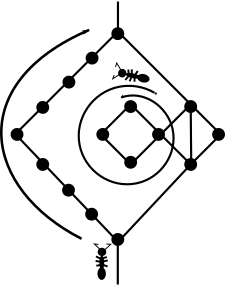
\includegraphics{extended_double_bridge}
\end{figure}
Skript s konstantní aktualizací měl dobré výsledky v grafech, kde není příliš mnoho kružnic. Příkladem nevhodného grafu je pak graf na obrázku \ref{fig:extendeddoublebridge}
Mravenci, kteří zůstanou v kružnicích, mohou dorazit do cíle tak pozdě, že mravenci kteří si vybrali delší, ale jednodušší cesty již provedli několik cest tam a zpět. I když na kružnice se díky jejich eliminaci neukládají žádné feromony, kolonie může v čase nutném ke zvýšení pravděpodobnosti na takových cestách, že mravenci v kružnicích nezůstávají, zkonvergovat k jednodušší, ale delší cestě.  Pokud by mravenci na sebe v cíli čekali před započetím zpáteční cesty, k tomuto problému by nedocházelo. 

Problém s kružnicemi částečně adresuje ohodnocení kvality cesty. Mravenci se sice v kružnicích zdrží, ale na delších cestách budou ukládat méně feromonů. Počet feromonů $\Delta \tau_{ij}^k$, které mravenec $k$ uloží na cestu $i, j$ jsme volili
\begin{equation}
\Delta \tau_{ij}^k = \frac{1}{ \left( C^k \right)^\gamma}
\end{equation}
kde $C^k$ je délka cesty mravence $k$ a $\gamma$ je koeficient, který nám dovoluje ovládat poměr krátkých$\times$dlouhých cest. 

\subsection{Implementace Ant System}
Protože se AS od S-ACO liší pouze v tom, že mravenci na sebe v cíli počkají, a aktualizace feromonů se provede pro všechny ve stejném čase, nebyl pro nás přechod od S-ACO k AS žádným problémem. Kvalita výsledků se ale v porovnání s S-ACO velmi zlepšila, zřejmě díky eliminaci vlivu zdržení mravenců smyčkami. Implementaci AS naleznete v souboru \texttt{ant\_system.rb}.

\subsection{Příklady použití skriptů}
Konstantní ohodnocovací funkce
\begin{verbatim}
require 'Graf.rb'
require 'minimum_cost_path.rb'
g = Graf.new(3, [[1, 2], [2, 3], [1, 3]])
# vyvtoříme kolonii, která se bude snažit v grafu g najít 
# nejkratší cestu ze zdroje 1 do cíle 3 pomocí 20ti mravenců
mcp = MinimumCostPath.new(g, 1, 3, 20)
# necháme všechny mravence popojít o 100 kroků
mcp.step_each 100
# podíváme se na pravděpodobnost, že mravenec, 
# který je v bodě 1 vybere hranu 1-3
mcp.p 1, 3, [1]
\end{verbatim}
Ohodnocovací funkce dle kvality cesty má stejné API, jen je třeba načíst soubor \texttt{minumum\_cost\_path\_weighted.rb}.

Ant System se nachází v souboru \texttt{ant\_system.rb}
\begin{verbatim}
require 'ant_system.rb'
as = AntSystem.new(g, 1, 3, 20)
# každý mravenec sestaví cestu 10krát a 10krát budou
# aktualizovány feromony
as.run 10
as.p 1, 3, [1]
\end{verbatim}

\section{Využití Ant System jako samoučícího algoritmu v deskové hře}
\subsection*{Co je to samoučící algoritmus pro deskovou hru}
V kontextu této práce budeme za samoučící považovat takový algoritmus pro deskovou hru, který se je schopen svou úspěšnost zvyšovat na základě odehraných her a přizpůsobovat se protihráči. 
\subsection{Desková hra}
Jako prototypovou deskovou hru jsme vybrali piškvorky na poli $3 \times 3$. Hru hrají 2 hráči na čtvercovém hracím poli rozděleném na 9 políček. Hráče označíme \emph{křížek} a \emph{kolečko}. Hru zahujeje křížek a hráči se střídají v umís\v{t}ování svých znaků na políčka. Hra končí v okamžiku, kdy se jednomu z hráčů podaří obsadit 3 pole v jedné linii, a\v{t} už diagonální, vertikální nebo horizontální. Hra končí remízou pokud jsou zaplněna všechna pole.

Tuto deskovou hru jsme vybrali pro její jednoduchost. Hra je dobře prozkoumána a optimální strategie je dobře známa. Je dokázáno, že bezchybnou hrou na straně obou hráčů vždy dojde k remíze \cite{ostermiller} \cite{tictactoegames}. 
\begin{figure}[btp]\caption{Hra piškvorky} \label{fig:tictactoe-gametree}
	\centering
	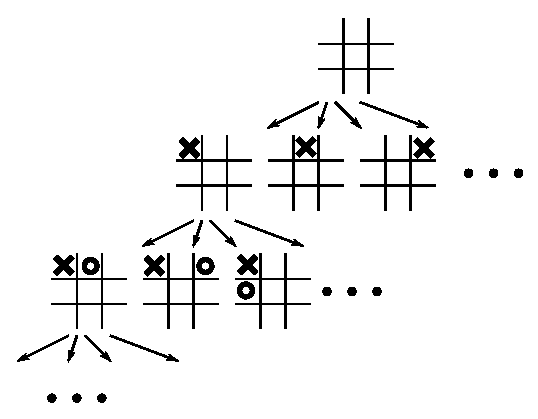
\includegraphics{tictactoe_game_tree}
\end{figure}

\subsubsection{Implementace deskové hry}
Hra se skládá ze dvou hlavních tříd, \texttt{Board} a \texttt{TicTacToe}. \texttt{Board} má na starosti implementaci hracího pole, \texttt{TicTacToe} se stará o pravidla a stavy hry. Hráči jsou nezávislé entity dědící ze třídy \texttt{Player}, které pro libovolný stav hry vyberou tah, který se má dle jejich názoru provést. K tomu mohou využít moduly s funkcemi pro ohodnocení desek, ohodnocení tahů a výběru nejlepšího tahu. Takováto architektura je velmi modulární a dovoluje nám případně jednoduše změnit hru (stačí místo třídy \texttt{TicTacToe} použít jinou se stejným API) a vytvářet nové hráče.

\subsection{Implementace tradičních algoritmů}
Jako zástupce tradičních algoritmů byl zvolen algoritmus MiniMax, konkrétně jeho varianta Negamax. MiniMax je rekurzivní algoritmus pro výběr dalšího tahu. MiniMax ohodnotí všechny stavy hry v určené hloubce stromu hry podle toho, jak moc je pro hráče žádoucí jich dosáhnout. Algoritmus pak vybere takový tah, který maximalizuje minimální hodnotu, které může hráč dosáhnout. Počet stavů, které musí MiniMax prozkoumat roste exponenciálně s počtem stavů které jsou dosažitelné jedním tahem. Proto neoptimalizované implementace MiniMaxu mají velkou časovou složitost. Výkon se dá jednoduše zvýšit pomocí alfa-beta ořezávání nebo jiných technik. 

\subsection{Implementace Ant System}
Jako konstrukční graf budeme používat graf, ve kterém vrcholy představují stavy hry a mezi dvěma vrcholy $i$ a $j$ je hrana pokud se dá ze stavu $i$ přejít do stavu $j$ jedním tahem a tento tah vyhovuje pravidlům. Z povahy hry v grafu nebudou žádné kružnice. Intuitivní představa takového grafu je znázorněna na obrázku \ref{fig:tictactoe-gametree}.
Jako zdroj budeme považovat výchozí stav hry, jako cíl jakýkoli stav s výhrou nebo remízou. Snažíme se pak nalézt nejbezpečnější cestu vedoucí k výhře nebo remíze. Jako běhy jednotlivých mravenců budeme používat skutečně odehrané hry. Po načtení počtu běhů rovného $m$ provedeme aktualizaci feromonů a jejich vyprchávání. Jako nejlepší tah z aktuální pozice pak zvolíme tah, který by si vybral imaginární mravenec nacházející se ve vrcholu konstrukčního grafu, který představuje tuto pozici.

Novou hru můžeme začít s už inicializovanými cestami na základě předchozího učení, tím dostane hráč paměť mezi hrami. Musíme si tedy ukládat globální pole feromonů ze kterého hráč vybírá tahy a lokální pole feromonů, do kterého jsou zapsány odehrané hry, které ještě nebyly přeneseny na pole globální.

\subsubsection{Program pro vytvoření učících dat}
Pro zajištění relevantnosti her používaných k naučení algoritmu jsme použili lidské hráče. Pro záznam jimi odehraných her jsme vytvořili jednoduchou grafickou utilitu \texttt{piskvorky-gui}. Utilita umožňuje hráčům zaznamenávat tahy kliknutím myši do hracího pole a dokončenou hru pak uložit a ukončit stisknutím tlačítka \texttt{save} nebo zahodit zavřením okna. Utilita nijak nehlídá pravidla hry, pouze střídá křížky a kolečka - předpokládáme, že hru oba hráči znají. K uložení odehraných her jsme použili knihovnu PStore, která nám dovoluje přistupovat do souboru jako do datové struktury Hash. Ukládáme do souboru \texttt{games.pstore} pod klíč \texttt{:games}.

\subsubsection{Zpracování učících dat}
Získaná data obsahují hry zakončené jak výhrou hráče \uv{křížek}, tak výhrou hráče \uv{kolečko}, tak remízy. Pro herní strategii jsme se rozhodli tato data zpracovat dvěma způsoby.

V prvním případě jsme do feromonové funkce zahrnuli jen tahy, které končí výhrou hráče, který začíná. Feromonovou funkci pak mají oba mravenci společnou, hráč kolečko ale vybírá tahy naopak jako hráč křížek. Vybírá tedy tahy nejméně vhodné pro hráče křížek. Tento způsob jsme zvolili na základě algoritmu NegaMax. Pravděpodobnost výběru cesty pro hráče kolečko jsme nemohli počítat prostě 
\begin{equation}\label{eq:as-impl-wrong-pravdepodobnost}
p_{ij}^\text{kolečko} = 1 -  p_{ij}^\text{křížek}
\end{equation}
protože suma pravděpodobností všech možných tahů by pak mohla být $\ge 1$. Proto jsme pravděpodobnosti spočtené dle \eqref{eq:as-impl-wrong-pravdepodobnost} považovali za poměrné části a dopočítali pravděpodobnost tak aby součet byl 1.

\begin{equation}
	\tau_{ij} \leftarrow \tau_{ij} + \sum_{k=1}^m \Delta \tau_{ij}^ {k} \qquad \forall(i,j) \in H
\end{equation}

\begin{equation}
	\Delta \tau_{ij}^{k} = \begin{cases} 
		0.5 	&\text{pokud hru vyhrál křížek}
	\\
		0.25 	&\text{pokud hra skončila remízou}
	\\
		0	 	&\text{jinak}
	\end{cases}
\end{equation}

\begin{equation} \label{eq:as-impl-pravdepodobnost-krizek}
	p_{ij}^{k \; \text{křížek}} =
		 \frac{(\tau_{ij})^\alpha(\eta_{ij})^\beta}
		 {\sum_{l \in S_{i}^{k}}(\tau_{il})^\alpha (\eta_{il})^\beta}
\end{equation}

\begin{equation} \label{eq:as-impl-pravdepodobnost-kolecko}
	p_{ij}^{k \; \text{kolečko}} = 
		\frac{ \left[1-p_{ij}^{k \; \text{křížek}} \right]^\gamma }
		{\sum_{l \in S_{i}^{k}} \left[1 - p_{il}^{k \; \text{křížek}} \right]^\gamma }
\end{equation}

\begin{equation}
  \eta_{ij} = \begin{cases}
    10		& \text{pokud tahem z $i$ do $j$ hráč křížek vyhraje}
    \\
    0.1    & \text{pokud tahem z $i$ do $j$ hráč křížek prohraje}
    \\
    5       & \text{jinak}
 \end{cases}
\end{equation}

Vyprchávání feromonů jsme použili stejné jako \eqref{eq:aco-aktualizace}. Argument $\rho$ jsme volili $0.5$, kterou uvádí \cite{maniezzo2004} jako obecně vhodnou hodnotu.

Zavedli jsme nový parametr $\gamma$, který slouží k zvýraznění rozdílu mezi pravděpodobnostmi pro hráče kolečko. Důvod můžeme ukázat na příkladě v tabulce \ref{tab:pravdepodobnost-problem}. V tabulce jsou zaneseny 4 různé tahy, ze kterých si kolečko vybírá. Tahy do $a, b, c$ jsou si rovny. Pravděpodobnost, kterou křížek přiřazuje tahu z $i$ do $d$ je velmi nízká, tedy hráč kolečko by ho měl velmi preferovat. S $\gamma = 1$ mu kolečko přiřazuje jen o málo vyšší pravděpodobnost než tahům $a, b, c$. S $\gamma$ vyšším jak 5 dostáváme pravděpodobnosti lépe modelující požadované chování hráče kolečko. 


\begin{table}[hbt]
  \caption{Problém s výpočtem pravděpodobností}
  $x_j = p_{ij}^{\text{křížek}} \\
  y_j = p_{ij}^{\text{kolečko}}$
  \begin{center} 
    \begin{tabular}{ | c | c|c | c|c | c|c | c|c |}
    
      \hline
	  $\gamma$ & \multicolumn{2}{c|}{ $x_a = 0.33$} & \multicolumn{2}{c|}{$x_b = 0.33$} & \multicolumn{2}{c|}{$x_c = 0.33$} & \multicolumn{2}{c|}{$x_d = 0.01$} \\ \hline
	           & $(1 - x_a)^\gamma$ & $y_a$ & $(1 - x_b)^\gamma$ & $ y_b$ & $(1 - x_c)^\gamma$ & $y_c$ & $(1 - x_d)^\gamma$ & $y_d$ \\ \hline
	  
	  1 & 0.67 & 0.22 & \ldots & \ldots  &  \ldots & \ldots   & 0.99 & 0.34 \\ \hline
	  2 & 0.45 & 0.20 & \ldots & \ldots  &  \ldots & \ldots   & 0.98 & 0.40 \\ \hline
	  3 & 0.30 & 0.16 & \ldots & \ldots  &  \ldots & \ldots   & 0.97 & 0.52 \\ \hline
	  4 & 0.20 & 0.13 & \ldots & \ldots  &  \ldots & \ldots   & 0.96 & 0.61 \\ \hline
 $\vdots$ & $\vdots$ & $\vdots$ & $\vdots$ & $\vdots$ & $\vdots$ & $\vdots$ & $\vdots$ & $\vdots$ \\ \hline
     10 & 0.02 & 0.02 & \ldots & \ldots  &  \ldots & \ldots   & 0.94 & 0.94 \\ \hline
	   \end{tabular}
    \label{tab:pravdepodobnost-problem}
  \end{center}
\end{table}

Parametr $\beta$ jsme volili 2. Díky funkci $\eta_{ij}$ se bude hráč křížek vyhýbat tahům, které vedou k prohře a silně preferovat tahy vedoucí k výhře. $\eta_{ij}$ pro výhru kolečka jsme volili nenulový se záměrem vyhnutí se dělení nulou v rovnici \eqref{eq:as-impl-pravdepodobnost-krizek}. Když bychom snížili hodnoty $\beta$ a $\eta{ij}$ pro výhru křížku, dostali bychom více chybujícího hráče. 

Druhým způsobem je samostatné ohodnocení pro prvního a druhého hráče. Hráči pak mají každý vlastní feromonovou funkci $\tau_{ij}^\text{kolečko}$ a $\tau_{ij}^\text{křížek}$, jejich aktualizace je také nezávislá. Funkci $\Delta \tau_{ij}^k$ jsme zvolili takovou, že hry které skončily prohrou příslušného hráče se do cest neprojeví. 

\begin{equation}
  \tau_{ij}^\text{křížek} \leftarrow \tau_{ij}^\text{křížek} + \sum_{k=1}^m \Delta \tau_{ij}^ {k},    \forall(i,j) \in H
\end{equation}

\begin{equation}
  \tau_{ij}^\text{kolečko} \leftarrow \tau_{ij}^\text{kolečko} + \sum_{k=1}^m \Delta \tau_{ij}^ {k},    \forall(i,j) \in H
\end{equation}

\begin{equation}
  \Delta \tau_{ij}^{k} = \begin{cases} 
    0.5 &\text{pokud hru vyhrál příslušný hráč}
    \\
    0.25 &\text{pokud hra skončila remízou}
    \\
    0 &\text{jinak}
  \end{cases}
\end{equation}

\section{Porovnání s klasickými algoritmy}

\begin{table}[tbh]
 \caption{Porovnání algoritmů - LOC}
\begin{small}
  \textit{LOC - Lines of Content}
\end{small}
 \begin{center}
   \begin{tabular}{|c|r|}
      \hline 
      Algoritmus & LOC \\ \hline  \hline
      Random & 1 \\ \hline 
      MiniMax & 7 \\ \hline 
      AntSystem & 197 \\ \hline 
    \end{tabular}
  \end{center}
  \label{tab:loc}
\end{table}

\subsection{Porovnání s algoritmem Random}
\subsubsection{Časová složitost}
Algoritmus Random vybírá tah náhodně, má tedy konstantní časovou složitost.
\subsubsection{Složitost implementace}
Algoritmus Random je implementačně jednoduchý.
\subsubsection{Kvalita hry}
Algoritmus Random hraje náhodně, tedy nedosahuje dobrých výsledků.


\subsection{Porovnání s algoritmem MiniMax}
\subsubsection{Časová složitost}
MiniMax zabere výběr tahu u velkých hloubek velmi mnoho času. Náš systém v porovnání s ním provede časově náročnou část (učení) v předstihu a při samotném výběru provede jen několik jednoduchých porovnání. Dodatečné učení z nově odehraných her je velmi rychlé.

\subsubsection{Složitost implementace}
Myslíme si, že ačkoli měření složitosti kódu pomocí počtu řádků není obecně příliš vypovídající, téměř 30ti násobný rozdíl je významný, viz. tabulka  \ref{tab:loc}.
MiniMax je implementačně velmi jednoduchý, v Ruby má jeho implementace jn 7 řádků (tabulka \ref{tab:loc}). Tak krátký algoritmus má výhodu, že se v něm případné chyby velmi jednoduše odhalují a opravují. Oproti tomu implementace \ac{AS} je poměrně složitá, a případná chyba je hůře odhalitelná. Proto jsme se u problémovějších částí drželi filozofie \ac{TDD}. \ac{TDD} předepisuje postupovat dle mantry \uv{red, green, refactor}, což znamená napsat testy pro ještě neexistující metody, které selhávají (red), implementovat metody, které testy splní (green) a nakonec metody refaktorovat do čitelnější nebo optimálnější podoby. Tento způsob psaní kódu je vhodný a běžný u dynamicky typovaných jazyků, kde chybí typová kontrola.
\subsubsection{Kvalita hry}
Kvalita hry algoritmu MiniMax je závislá od hloubky, do které prohledává pozice. Od hloubky hledání je závislý i čas výpočtu. Musíme tedy kvalitu hry a čas pro výpočet vyvažovat. U námi zvolené hry piškvorky je pro vítězství kritické vybrat dobrý první tah (střed nebo roh). Takovéto úvahy ale MiniMax není schopen. Zárove\v{n} se MiniMax nemůže poučit z chyb. Pokud hráč najde strategii při které je vynucená výhra až za \uv{horizontem} MiniMaxu, MiniMax takovéto strategii vždy podlehne. Kvalita hry MiniMaxu záleží téměř výhradně na ohodnocovací funkci. Pokud je taková funkce bez vlivu náhody, MiniMax bude hrát vždy stejně.

%%% Závěr práce v~češtině
\begin{conclusions-cz}
Algoritmy z rodiny Ant Colony Optimalization jsou dobrou alternativou pro řešení grafových úloh. Podařilo se nám implementovat třídu, o které si myslíme, že je dobrou alternativou k algoritmu MiniMax. Co se týče volby piškvorek jako hry pro demonstraci možností, myslíme si, že volba byla správná. 

V implementaci algoritmu je mnoho prostoru pro zlepšení. Například bychom mohli zrcadlově stejné hry slučovat pod jednu a podobně. Tím by se snížila šířka stromu. Myslíme si ale, že třída poskytující algoritmu je napsána tak aby byla jednoduše upravitelná pro jiné hry.
\end{conclusions-cz}


%%% Závěr práce v~angličtině
\begin{conclusions-en}
  Conclusion in english. 
\end{conclusions-en}


%%% Vytvoření seznamu literatury.
\newpage
\bibliographystyle{czechiso}
\bibliography{bakalarka}

%%% Přílohy.
\newpage
\appendix

\section{První příloha} \label{PrvniPriloha}
Závěrečné poznámky, k~programování.

\newpage
\section{Obsah přiloženého CD} \label{ObsahCD}
V~samotném závěru práce je uveden stručný popis obsahu přiloženého
CD/DVD, tj. závazné adresářové struktury, důležitých souborů apod.

\begin{description}

\item[\texttt{bin/}] \hfill \\
Instalátor \textsc{Instalator} programu a další program
\textsc{Program} spustitelné přímo z CD/DVD. / Kompletní adresářová
struktura webové aplikace \textsc{Webovka} (v ZIP archivu) pro
zkopírování na webový server. Adresář obsahuje i všechny potřebné
knihovny a další soubory pro bezproblémové spuštění programu / pro
bezproblémový provoz na webovém serveru.

\item[\texttt{doc/}] \hfill \\
Dokumentace práce ve formátu PDF, vytvořená dle závazného stylu KI PřF
pro diplomové práce, včetně všech příloh, a všechny soubory nutné pro
bezproblémové vygenerování PDF souboru dokumentace (v ZIP archivu),
tj. zdrojový text dokumentace, vložené obrázky, apod.

\item[\texttt{src/}] \hfill \\
Kompletní zdrojové texty programu \textsc{Program} / webové aplikace
\textsc{Webovka} se všemi potřebnými (převzatými) zdrojovými texty,
knihovnami a dalšími soubory pro bezproblémové vytvoření spustitelných
verzí programu / adresářové struktury pro zkopírování na webový server
(v ZIP archivu).

\item[\texttt{readme.txt}] \hfill \\
Instrukce pro instalaci a spuštění programu \textsc{Program}, včetně
požadavků pro jeho provoz. / Instrukce pro nasazení webové aplikace
\textsc{Webovka} na webový server, včetně požadavků pro její provoz, a
webová adresa, na které je aplikace nasazena pro testovací účely a pro
účel obhajoby práce.

\end{description}

Navíc CD/DVD obsahuje:

\begin{description}

\item[\texttt{data/}] \hfill \\
Ukázková a testovací data použitá v práci a pro potřeby obhajoby
práce.

\item[\texttt{install/}] \hfill \\
Instalátory aplikací, knihoven a jiných souborů nutných pro provoz
programu / webové aplikace, které nejsou standardní součástí operačního
systému.

\item[\texttt{literature/}] \hfill \\
Některé položky literatury odkazované z dokumentace práce.

\end{description}

U veškerých odjinud převzatých materiálů obsažených na CD/DVD jejich
zahrnutí dovolují podmínky pro jejich šíření nebo přiložený souhlas
držitele copyrightu. Pro materiály, u kterých toto není splněno, je
uveden jejich zdroj (webová adresa) v textu dokumentace práce nebo v
souboru \texttt{readme.txt}.

\end{document}
